\documentclass[11pt, a4paper]{article}
\usepackage[main=galician, spanish]{babel}
\usepackage{fontspec}
\usepackage{libertinus}%%automatically loads aunicode-math package
%%\renewcommand{\familydefault}{\sfdefault}
\usepackage{float}
\usepackage{parskip}
\usepackage[version=4]{mhchem}
\usepackage[figuresleft]{rotating}
\usepackage{graphicx}
\usepackage{amsmath}
\usepackage{slashed}
\usepackage{wrapfig}
%\usepackage{amsfonts}
%\numberwithin{equation}{section}%%numbering eqs by section
\usepackage{fancyhdr} 
\usepackage[dvipsnames, table]{xcolor}
\usepackage{wrapfig}
\usepackage[labelfont=bf, skip=4pt, figureposition=bottom, font=normalsize]{caption}
\usepackage{siunitx}
\usepackage{adjustbox}
\usepackage{booktabs} 
\usepackage{multirow}
\usepackage[a4paper,left=2cm,right=2cm,top=2.5cm,bottom=2.5cm]{geometry}
\usepackage{csquotes}
\usepackage{enumitem}
\usepackage{subcaption}
\usepackage{listings}
\usepackage{abstract}
\usepackage{hyperref} 
%%adapted to galician (GZ)
\renewcommand{\tableautorefname}{Cadro}
\usepackage{lipsum}

%% ENUMITEM settings
%\setlist{itemsep=4pt}
\setlist[enumerate,1]{
  label={\bfseries \arabic*.},
}

%% SIUNITX
\sisetup{output-decimal-marker = {,}}
\sisetup{exponent-product= \cdot}
\sisetup{separate-uncertainty=false}
\sisetup{table-parse-only=true}
\sisetup{inter-unit-product = \ensuremath { { } \cdot { } } }
\sisetup{detect-all}
\sisetup{group-digits=integer}
\sisetup{print-unity-mantissa=false}
\sisetup{list-final-separator = { e }}
\sisetup{range-phrase = -}
\sisetup{range-units = single}
\sisetup{list-units = single}
\sisetup{propagate-math-font = true}
\sisetup{text-series-to-math = true}
\sisetup{list-final-separator = { e }}
\sisetup{list-pair-separator = { e }}
\DeclareSIUnit{\espesor}{\milli\g\per\cm\squared}
\DeclareSIUnit{\aten}{\cm\squared\per\milli\g}
\DeclareSIUnit\clight{\text{\ensuremath{c}}}
\DeclareSIUnit\year{a}
\DeclareSIUnit{\barn}{b}
\DeclareSIUnit{\bar}{bar}
\DeclareSIUnit{\neutrons}{\text{neutróns}}
\DeclareSIUnit{\deuterons}{\text{deuteróns}}
\DeclareSIUnit{\counts}{\text{contas}}

%%OTHER COMMANDS
%% for isotopes
\newcommand{\iso}[2]{\ce{^{#1}#2}}
%for vectors
\newcommand{\vect}[1]{\boldsymbol{#1}}
%for ann
\newcommand{\ann}{a_{nn}}
% figure sizes
\newcommand*{\fw}{0.6}
%%for lstlisting package
\definecolor{backcolour}{rgb}{0.95,0.95,0.92}
\lstset{
%backgroundcolor=\color{backcolour},
basicstyle=\small\ttfamily,
language=python,
keepspaces=false,
keywordstyle=\bfseries\color{Purple},
morekeywords={TSpectrum, TH1, TH1I, TH1D,
Double_t, Int_t, TGraph, TGraphErrors, TMinuit, TF1, TSpline3, G4NistManager,
QGSP_BIC_HP,
SimGeometry, ROOT, Math, XYZPoint, XYZVector, SRIM},
stringstyle=\color{Orange},
identifierstyle=\color{ForestGreen},
breaklines=false,
captionpos=b,
belowskip=-0.85 \baselineskip,
%columns=flexible,
}

\title{\textbf{Guión das prácticas no IGFAE}}
\author{%Miguel Lozano González\\
\small{Prácticas optativas de Grao $\cdot$ Curso 24-25}\\
\small{Universidade de Santiago de Compostela}}
\date{\empty}%\date{\today}

\pagestyle{fancy}
\fancyhf{}
%\fancyhead[R]{\thepage}
\fancyhead[R]{\textsc{guion prácticas igfae}}
\fancyfoot[C]{\thepage}
\renewcommand{\headrulewidth}{0.75pt}
%\renewcommand{\footrulewidth}{0.75pt}
\setlength{\headheight}{14.5pt}

\hypersetup{
	colorlinks=true,
    linkcolor=blue,
    filecolor=magenta,      
    urlcolor=cyan,
}

%% BIBLIOGRAPHY
% \usepackage[
% backend=biber,
% style=numeric,
% sorting=none
% ]{biblatex}
% \addbibresource{./biblio.bib}

%% DOCUMENT

\begin{document}
\begin{minipage}{0.48\linewidth}
    \maketitle
\end{minipage}\hfill
\begin{minipage}{0.48\linewidth}
    \tableofcontents
\end{minipage}

\noindent\rule{\textwidth}{1pt}
% {\renewcommand{\abstractname}{}
% \renewcommand{\absnamepos}{empty}
% \begin{abstract}
% \noindent Memoria das prácticas externas do Mestrado en Física realizadas no Grupo de Física Corpuscular e Aplicacións (FICA), adscrito ao IGFAE (\url{https://igfae.usc.es/igfae/}), baixo a supervisión de Juan Lois Fuentes (\url{juan.lois.fuentes@usc.es}), sendo titora académica Beatriz Fernández Domínguez (\url{beatriz.fernandez.dominguez@usc.es}).
% \end{abstract}
% }
\section{Presentación}
\subsection{Obxectivos}
O obxectivo destas prácticas vai ser de introducir técnicas de \textit{machine learning} na análise de datos do detector \textit{ACtive TARget and Time Projection Chamber} (ACTAR TPC). Máis concretamente, centrarémonos en identificar as partiículas de alta enerxía que superan dous muros de silicio. Trátase dunha técnica novel que nunca se implementou neste tipo de dispositivos, polo que non está garantido que funcione... Pero merece a pena probar e pode ofrecer unha formación moi interesante.

Abarcaremos varias áreas:
\begin{itemize}
    \item \textbf{Programación}: Afondaremos na programación con \verb|python|, utilizando módulos de \textit{ML} como \verb|tensorflow| ou \texttt{scikit-learn}. Melloraremos os coñecementos de \verb|pandas| e \verb|matplotlib|, así como unha introdución aos \textbf{histogramas} con \verb|hist|.

    \item \textbf{Detectores}: ACTAR TPC é un detector gasoso moi recente que abre todo unha nova ventá de posibilidades no eido das reaccións nucleares. Introduciremos os conceptos básicos dun detector gasoso e complementarémolos cos de detectores de silicio, esenciais neste experimento.

    \item \textbf{Teoría}: Expoñeremos as leis básicas da cinemática que rixen calquera reacción entre partículas e introduciremos os fundamentos da interacción radiación-materia, básicos neste experimento.
\end{itemize}

Comezaremos estudando os fundamentos teóricos e implmentándoos manualmente para asegurar que se entenden ben. A segunda parte abarcará a parte computacional en si mesma, tentando chegar ao obxectivo final de identificar as partículas.

\subsection{Motivación}
Este ano levarase a cabo un experimento para estudar reaccións de transferencia co \iso{11}{Li}, de xeito que se poda facer un estudo pormenorizado da súa estrutura nuclear. Estudos coma este son moi importantes, posto que o \textit{modelo de capas nuclear} (moi parecido ao seu análogo atómico) sábese que falla a medida que nos afastamos da estabilidade e pasamos a outros núcleos máis exóticos ($N / Z \gg 1$), e faise necesario postular modelos teóricos máis amplos, válidos de forma xenérica.

As reaccións que imos estudar son:
\begin{itemize}
    \item $\iso{11}{Li} + \iso{}{d} \rightarrow \iso{}{p} + \iso{12}{Li}$

          É unha reacción de engádega dun neutrón.

    \item $\iso{11}{Li} + \iso{}{d} \rightarrow \iso{}{d} + \iso{11}{Li}$

          É a difusión elástica (E$_{x} = 0$) ou inelástica (E$_x > 0$).

    \item $\iso{11}{Li} + \iso{}{d} \rightarrow \iso{}{t} + \iso{10}{Li}$

          Aquí, ao contrario, eliminamos un neutrón.
\end{itemize}

Todo isto é posíbel grazas á seguinte configuración do detector:
\begin{itemize}
    \item \textbf{Gas}: O gas que encherá ACTAR TPC será unha mestura de \ce{D_2} e \ce{CF_4} (\qty{90}{\percent} e \qty{10}{\percent}, respectivamente) a unha presión de \qty{900}{\milli\bar}. Será o \ce{D_2} o que provea os $\iso{}{d}$ da reacción.
    \item \textbf{Feixe}: O \iso{11}{Li} terá unha enerxía de \qty{7.5}{A\MeV} (é dicir, \qty{82.5}{\MeV}), e será producido no acelerador ISAC de TRIUMF, en Canadá.
\end{itemize}

\section{Principios físicos}
\subsection{Un detector gasoso}
ACTAR TPC segue os principios de funcionamento dunha \textit{time projection chamber}: as partículas ao pasaren polo gas ionizan os átomos, liberando electróns que \textbf{derivan} baixo aplicación dun campo eléctrico. Esta carga é recollida nun sensor amplamente fragmentado (\textit{pad plane}), permitindo \textit{seguir} as partículas no seu traspaso dentro do medio en 2D.

Pero é máis: pódese engadir a terceira coordenada coñecendo o tempo que lle leva aos electróns chegar ao \textit{pad plane}, pois a \textbf{velocidade de deriva} é constante. Deste xeito, o seguimento das partículas faise en \textbf{3D}.

Finalmente, o principio de \textit{active target} engade a vantaxe de ser o gas o propio albo da reacción: este actúa como medio de reacción e de detección. O seguinte esquema ilustra este modo de funcionamento.
\begin{figure}[!ht]
    \begin{minipage}[b]{.45\textwidth}
        \centering
        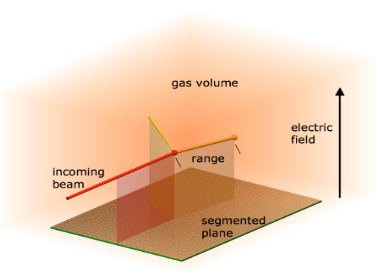
\includegraphics[width=1\textwidth]{figures/tpc.png}
        \caption{Esquema de funcionamento dunha TPC.}
        \label{fig:tpc}
    \end{minipage}
    \hfill
    \begin{minipage}[b]{.45\textwidth}
        \centering
        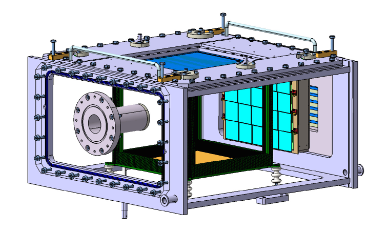
\includegraphics[width=1\textwidth]{figures/actar.png}
        \caption{Deseño do detector ACTAR TPC. A rexión de detección é a parte negra interna.}
        \label{fig:actar}
    \end{minipage}
\end{figure}

Os datos que vas analizar proveñen dunha simulación na cal se implementaron os seguintes parámetros:
\begin{itemize}
    \item O tamaño da zona de detección (\autoref{fig:actar}) é de \qtyproduct[product-units=power]{256 x 256 x 255}{\mm}.
    \item O criterio de dimensións é que o beam vai no eixo X, e a dimensión vertical é Z.
    \item Os detectores auxiliares poden poñerse arredor desta zona nos diferentes lados. Nós usaremos algo parecido ao da figura, cos detectores de Si (como os \textcolor{blue}{azuis}) cara adiante.
    \item Teremos dous muros de silicio, un tras do outro. O primeiro está a \qty{10}{\cm} do \textit{pad plane} e o segundo está separado do primeiro \qty{3}{\cm}. Cada muro constitúese de 12 unidades de tamaño \qtyproduct[product-units=power]{80 x 50 x 1.5}{\mm}.
\end{itemize}

A disposición xeométrica é a que se amosa a continuación.
\begin{figure}[!htb]
    \centering
    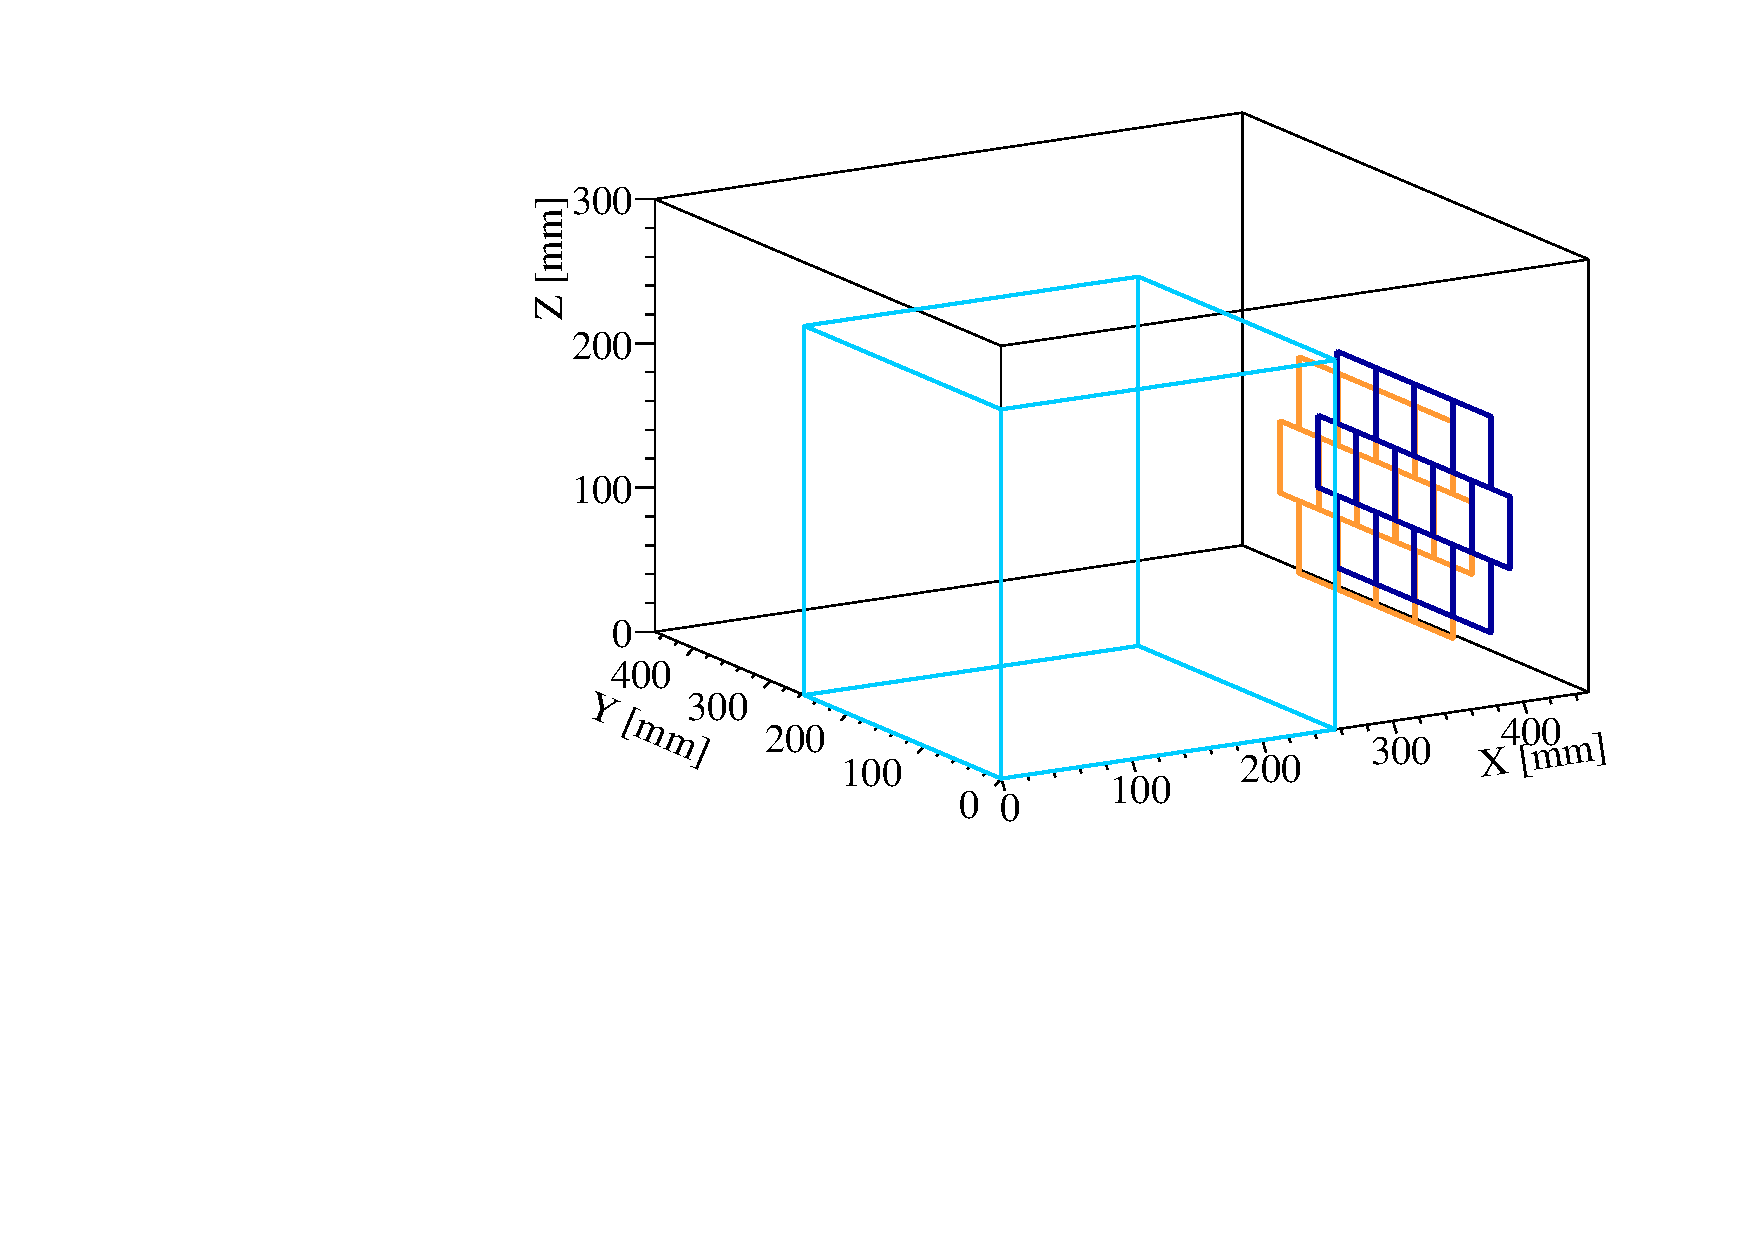
\includegraphics[width=0.7\linewidth]{figures/geo.pdf}
    \caption{O código de cores é o seguinte: \textcolor{Cyan}{ACTAR TPC en azul}, en \textcolor{Blue}{escuro a primeira capa de silicios} e en \textcolor{orange}{laranxa o segundo}.}
\end{figure}

\subsection{Perdas de enerxía na materia}\label{sec:de}
As partículas ao propagarse a través do gas interaccionarán co campo de Coulomb dos átomos deste, perdendo enerxía e liberando electróns. Esta perda de enerxía en cada interacción é moi pequena, pero como é moi elevado o número de colisións no gas (é, polo tanto, un proceso estocástico), chega a ser moi importante. Nunha aproximación continua, está dada pola \textbf{ecuación de Bethe-Bloch}:
\begin{equation*}\label{eq:stopping}
    - \frac{dE}{dx} \cong \frac{4 \pi e^4}{m_e} \left(\rho \frac{N_A}{M}\right)\frac{z^2 Z}{v^2} \ln{\frac{2m_e v^2}{I}}
\end{equation*}
Depende esencialmente da partícula a considerar ($Z$ e $A$) e do gas (a través de $\rho$). É interesante definir:
\begin{itemize}
    \item Rango ($R$): É o camiño percorrido por unha partícula ata que \textit{case} se detén. É función da enerxía inicial e do material a atravesar. Existe unha \textbf{relación unívoca} $E \Longleftrightarrow R$ que imos utilizar para estimar a perda da enerxía en función da distancia percorrida pola partícula.
    \item \textit{Straggling}: Como a perda de enerxía é un \textbf{proceso estatístico}, dúas partículas coa mesma enerxía inicial non van depositar a mesma $\Delta E$. O \textit{straggling} mide, dalgunha forma, a $\sigma$ desta distribución.
\end{itemize}
Esta información está tabulada nun programa que se coñece como \textit{\textbf{SRIM}} e que foi empregado para obter os datos que se analizarán. Non obstante, vas familiarizarte con el para entender ben os conceptos da interación radiación-materia introducidos.

\subsection{Detectores de silicio}

\begin{wrapfigure}{r}{0.4\textwidth}
    \begin{center}
        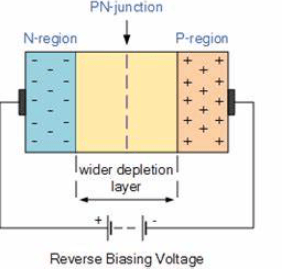
\includegraphics[width=0.7\linewidth]{figures/pn_junction.png}
    \end{center}
    \caption{Esquema dunha unión PN polarizada en inversa}
\end{wrapfigure}
Vas estudar os seus principios de funcionamento o próximo curso en \textit{Electrónica Física}, pero aquí tes unhas nocións básicas sobre o seu funcionamento. Cada silicio funciona como unha \textbf{unión PN}, na cal algúns átomos da rede cristalina de Si se subsituíron por outros: na rexión \textit{P}, por átomos deficitiarios en electróns (hai máis \textit{ocos}), mentres que na \textit{N} por outros ricos en $e^-$. Ao xuntalos créase unha zona interna de campo eléctrico pola diferenza de cargas, o que se coñece como \textit{zona de baleirado} ou de \textit{carga espacial}, e que ten un tamaño típico de \unit{\micro\m}.

Baixo a aplicación dun potencial apropiado, nunha configuración que se coñece como \textit{polarización inversa}, esta zona de baleirado faise moi grande, ocupando case todo o detector. E isto é o que nos interesa: as partículas cargadas, ao atravesar esta rexión, ionizan o medio liberando pares electrón-oco. Grazas ao campo eléctrico interno da unión PN podemos recollelos (os $e^-$) e medilos como correcte eléctrica. O sinal recollido é proporcional ao número de electróns liberados na ionización e, polo tanto, á enerxía incidente da partícula.

\subsection{Incertezas experimentais}
Como xa comentamos, os datos que se analizarán non proveñen dun experimento real senón dunha simulación. Non obstante, esta ten en conta os defectos experimentais implementables nun computado e que son determinantes en moitos casos do éxito ou non dun experimento. Aquí unha lista:
\begin{itemize}
    \item O \textit{straggling} en enerxía da partícula ao propagarse no gas.
    \item O mesmo pero ao propagarse no silicio.
    \item A \textbf{resolución} dos detectores de silicio. Na Sección anterior comentamos que a corrente medida é proporcional ao número de electróns de ionización xerados no proceso. Non obstante, a estatística gaussiana asígnalle unha interteza $u = \sqrt{N_e}$, o cal quere dicir que unha partícula coas mesmas características que atravese o Si non vai necesariamente rexistrar a mesma $\Delta E$. Experimentalmente mídese e estímase en \qty{50}{\keV} de incerteza a unha enerxía incidente de \qty{5.5}{\MeV}.
\end{itemize}

% Unha pequena apreciación: SRIM vainos dar o \textit{straggling} en posición, mais nós deberémolo converter a en enerxía. Aquí o algoritmo que imos usar:
% \begin{enumerate}
%     \item Calculamos $R_{ini}$ coa enerxía inicial, xunto co seu \textit{straggling}.
%     \item Sabendo que a partícula percorre unha distancia $d$ o rango nese punto será $R_{L} = R_{Ini} - d$. Avaliamos o \textit{stragg.} para este valor.
%     \item O \textit{straggling} na distancia estará \textbf{correlacionado con ambos}, e sabendo que $u^2(R_{Ini}) = u^2(R_{Left}) + u^2(d)$, despexamos $u(d)$.
%     \item Aleatorizamos o valor de $d$ cunha gaussiana centrada no seu valor e de $\sigma = u(d)$. Recalculamos o valor de $R_{Left} \longrightarrow R_{Left}^{\prime}$ coa nova $d \longrightarrow d\prime$.
%     \item Con este novo rango calculamos a enerxía final, efectivamente implementando o \textit{straggling}!
% \end{enumerate}


% \subsection{Resolución en enerxía}\label{sec:res}
% Complementariamente acostuman situarse detectores de Si que nos van permitir medir a enerxía das partículas á súa saída do \textit{pad plane} (seguindo os mesmos principios que na anterior Sección). Un parámetro importante destes é a \textbf{resolución en enerxía}, definida como a capacidade para \textit{resolver} enerxías depositadas distintas: $R = \textrm{FWHM} / E$.

% Para o noso experimento, esta resolución está tabulada en \qty{50}{\keV} a \qty{5.5}{\MeV} e podemos extrapolala ao resto de enerxías coa función:
% \begin{equation*}
%     R = \frac{2.35 \sigma}{E} = \frac{K}{\sqrt{E}} \quad \implies \quad \sigma = \frac{K}{2.35}\sqrt{E} = \frac{\qty{0.0213}{\MeV}}{2.35} \sqrt{E}
% \end{equation*}
% Isto vai significar que a perda de enerxía $\Delta E$ que calcules nos Si deberala aleatorizar cunha gaussiana de $\sigma$ obtida coa anterior fórmula.

\subsection{Cinemática}
Todo proceso de interacción entre partículas podes escribirse en termos de variables cinemáticas (enerxías e ángulos) usando as \textbf{leis de conservación} de enerxía e de momento. Esta pode ser descrita no sistema LAB ou no CM (mediante unha transformación Lorentz a un sistema con 3-momento nulo en ambas canles de entrada e saída) do seguinte xeito:

\begin{equation*}
    \begin{gathered}
        \text{No LAB:  }p_1=\left(E_1, \vect{p_1}\right); \; p_2=\left(m_2, \vect{0}\right); \; p_3=\left(E_3, \vect{p_3}\right); \; p_4=\left(E_4, \vect{p_4}\right) \\
        \text{No CM:  }p'_1=\left(E'_1, \vect{p'_1}\right); \;  p'_2=\left(E'_2, -\vect{p'_1}\right); \; p'_3=\left(E'_3, \vect{p'_3}\right); \; p'_4=\left(E'_4, -\vect{p'_3}\right)
    \end{gathered}
\end{equation*}

É estándar asumir unha partícula \textit{target} (a 2) en repouso. Aínda que a simulación xa está feito, penso que é interesante que comprendas como se xeran os eventos. Para iso, vas resolver as ecuacións de cinemática para obter a representación $T$ vs $\theta$ da partícula 3 que mediremos nós. Para iso:
\begin{itemize}
    \item Partiremos da enerxía cinética $T_1$ do feixe (1) no LAB.
    \item Calcularás a transformación Lorentz da canle de entrada ao CM.
    \item Repartiremos a $E_{CM}$ (enerxía total no centro de masas) entre as partículas de saída en función de $\theta_{CM}$ e $\phi_{CM}$.
    \item Finalmente, recuperaremos as enerxías de saída de ambas partículas no LAB coa transformación inversa.
    \item Tamén necesitaremos os ángulos no laboratorio, $\theta_{Lab}$ e $\phi_{Lab} = \phi_{CM}$.
\end{itemize}

Algunhas fórmulas que che poden ser interesantes para unha transformación Lorentz en X (o feixe móvese nesa dirección; é un convenio):
\begin{gather*}
    E^{\prime} = \gamma \left(E - \beta p_x\right), \qquad p^{\prime}_{x} = \gamma \left(p_x - \beta E\right)\\
    E = \gamma \left(E^{\prime} + \beta p_{x}^{\prime}\right), \qquad p_x = \gamma \left(p^{\prime}_x + \beta E^{\prime}\right)
\end{gather*}
Onde as variables primadas indican que son no CM. Cando transformes ao final do CM ao LAB terás en conta $\theta_{CM}$: $p_{3,x}^{\prime} = |\vect{p^{\prime}_3}| \cdot\cos(\theta_{CM})$. O ángulo $\phi_{CM}$ non aparece de momento posto que é transversal á transformación.

\section{Para comezar}
\subsection{Instalación de paquetes}
Para poder realizar esta análise imos necesitar unha serie de paquetes de \textit{python}:
\begin{enumerate}
    \item Crea un entorno virtual para esta análise, así non modificaremos nada da túa instalación actual. Segue as instrucións de \href{https://docs.python.org/3/library/venv.html}{aquí}.
    \item Unha vez dentro do teu \textit{venv}, instala os paquetes básicos: \verb|numpy|, \verb|matplotlib|, \verb|pandas|
    \item Instala \href{https://uproot.readthedocs.io/en/stable/basic.html}{\texttt{uproot}}. É un paquete que nos vai permitir ler os ficheiros de simulación creados en formato \verb|.root|
    \item Instala o paquete \href{https://github.com/loopset/PyPhysics}{\texttt{PyPhysics}} que che ofrecerá moitas clases de interese (cinemática e perdas de enerxía). Clona o repositorio e modifica o teu \verb|PYTHONPATH|.
\end{enumerate}



\subsection{Github}
Git é unha ferramenta de control de versións que che permitirá manter un historial do teu código, podendo volver atrás cando sexa necesario. Github é unha web para almacenar repositorios Git. Vamos utilizala para manter o código seguro nun servidor e volver cara atrás cando sexa necesario.

Para iso, o primeiro é ter unha conta en \url{www.github.com}. Tras unha configuración inicial un pouco tediosa, o plan de traballo é o seguinte, que se debe executar cando fagas cambios importantes ou cando remates a túa sesión de traballo:
\begin{enumerate}
    \item \lstinline|git add .| vai engadir todos os cambios dende o anterior \textit{commit}
    \item \lstinline|git commit| abrirá un editor de texto no que crear unha mensaxe para informar dos cambios. Péchase con \lstinline|Ctrl+S, Ctrl+X|
    \item \lstinline|git push| envía os cambios á nube
\end{enumerate}

No tocante ao paquete \texttt{PyPhysics}, probablemente teremos que actualizalo ao longo das prácticas. Para recibir os cambios do servidor, vai á carpeta na que está descargado e executa \verb|git pull|. Desta forma teralo actualizado.


\section{Plan de traballo}
Este é o plan de traballo das próximas semanas.

\begin{itemize}
    \item \textbf{Primeira semana}: Instalación de paquetes e familiriziación co entorno. Representación de todas as variables da simulación e das súas correlacións. Estudo da cinemática e das perdas de enerxía.
    \item \textbf{Segunda semana}: Preparación dos datos para entrenar unha rede neuronal. Comprensión do funcionamento destas e implementación dunha simple.
    \item \textbf{Terceira semana}: Engédega da rede neuronal convolucional 1D á anterior para analizar os perfís de carga. Ver se isto mellora os resultados. \textit{Fine-tuning} dos hiperparámetros.
    \item \textbf{Cuarta semana}: Análises complementarias e propostas doutras solucións en caso de que non funcione. Redacción da memoria de prácticas.
\end{itemize}

\subsection{Primeira semana}
Imos comezar por representar todas as variables que nos dá a simulación. Para iso empregaremos histogramas, que podes construír usando o módulo \verb|hist|.

\begin{lstlisting}
    import hist
    ## histograma 1D
    h1d = hist.Hist.new.Reg(nbinsx, xmin, xmax, label="X axis").Double()
    ## histograma 2D: hai que especificar ambos eixos
    h2d = hist.Hist.new.Reg(nbinsx, xmin, xmax, label="X axis")
                        .Reg(nbinsy, ymin, ymax, label="Y axis").Double()

\end{lstlisting}
Xunta todos os ficheiros nun único dataframe e representa:

\begin{itemize}
    \item A cinemática: $T_3$ vs $\theta_3$. deberías ver 3 liñas ben diferenciadas
    \item As perdas de enerxía nos silicios: $\Delta E_0$ vs $\Delta E_1$. É o que se coñece como \textit{Particle IDentification, (PID)}.
    \item A coordenada X do punto de reacción \verb|RPx|
    \item Colle un perfil de carga de cada reacción e compáraos
\end{itemize}

O seguinte paso vai ser entender o que vemos:
\begin{enumerate}
    \item Fai os cálculos de cinemática para obter a liña téorica para as tres reaccións: $\iso{11}{Li}(\iso{}{d},\iso{}{p}), (\iso{}{d}, \iso{}{d}), (\iso{}{d}, \iso{}{t})$. Podes intentar facer unha \textbf{clase} en \verb|python|.
    \item Empregando a clase \verb|EnergyLoss| de \verb|PyPhysics| fai propagar $\iso{}{p},\iso{}{d},\iso{}{t}$ unha mesma distancia no gas para distintas enerxías. Estuda o que vés e intenta explicalo a partir da fórmula de Bethe-Bloch.
    \item Explica porque hai moitas máis contas de \verb|RPx| cara ao final da TPC.
\end{enumerate}

\subsection{Segunda semana}
Agora imos aprender o que é unha rede neuronal e os conceptos básicos do \textit{machine learning}.
\begin{enumerate}
    \item Usa o Capítulo 2 de \textit{Hands-on Machine Learning with Scikit-Learn and Tensorflow} para ter unha idea de como debes tratar os datos. Aquí van algunhas suxestións:
          \begin{itemize}
              \item Crea un único dataframe con \textit{labels} indicando se é $p,d,t$
              \item Downsample os datos de forma que haxa o mesmo número de eventos de cada reacción
              \item Aleatoriza o \verb|df|
              \item Decide que \textit{features} debes eliminar: a $T_3$ claramente, pois se non permitiría unha distinción absoluta entre as partículas. Pensa que experimentalmente non é accesible sen identificar antes a partícula medida. Por outra banda, os perfís de carga deixarémolos para máis adiante.
              \item Normaliza as \textit{features}
              \item Encodifica as variables de clasificación: de strings a enteiros
              \item Dívideo en \textit{train} e \textit{validation}
          \end{itemize}
    \item Le as \textit{Lectures} da U. Cornell para entender o que é unha rede neuronal e en que consiste o proceso de entrenamento. A idea coa que debes reter sobre unha rede neuronal é que é un conxunto de funcións as cales, a partir duns parámetros de entrada (\textit{features}), aplican unha serie de transformacións (\textit{weights} + \textit{activation function}) para devolver unha saída. No noso caso, esta é unha clasificación: probabilidade de que sexa $p,d,t$.
    \item Cando metamos a rede convolucional estaría ben que leses os capítulos 6 e 7 das \textit{Lectures} da U. Pennsylvania. A nosa rede convolucional será 1D (un histograma) en lugar de 2D (unha imaxe), pero os conceptos son os mesmos.
\end{enumerate}

De seguido imos construír o noso primeiro modelo de rede neuronal. Na seguinte Figura tes un exemplo.
\begin{figure}[!htb]
    \centering
    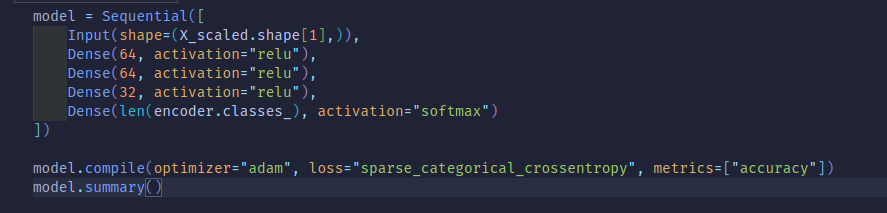
\includegraphics[width=0.8\linewidth]{figures/basic_model.png}
    \caption{Modelo básico de rede neuronal para clasificación.}
\end{figure}

Algunhas apreciacións:
\begin{itemize}
    \item Usamos activación \textit{softmax} na layer de saída para clasificación non binaria (hai 3 clases de saída)
    \item A función a minimizar é a \textit{cross entropy}, tamén adecuada para estas tarefas
\end{itemize}
Axusta o modelo e plotea a fit accuracy por epoch, así como a matrix de confusión. Podes representar outras métricas, como a precision ou a recall. Le o Capítulo 3 do libro para máis información.

Podes probar outras arquitecturas da rede, con outras funcións de activación ou optimizadores (Capítulo 11, \textit{Optimizers} do libro) a ver se atopas unha combinación que ofreza unha mellor exactitude.

Por último, no plot do PID superimpón os eventos mal identificados e que ideas se che ocorren para explicalo.

\subsection{Terceira semana}
Finalmente, intentaremos mellorar a rede neuronal introducindo os perfís de carga, pois como xa viches son característicos de cada partícula, polo que poderían axudar moito na clasificación. Para iso deberemos combinar a rede neuronal simple anterior cunha convolucional 1D, pois non se trata dunha imaxe senón dunha serie de valores de $d\text{E}/d\text{x}$.
\begin{figure}[!htb]
    \centering
    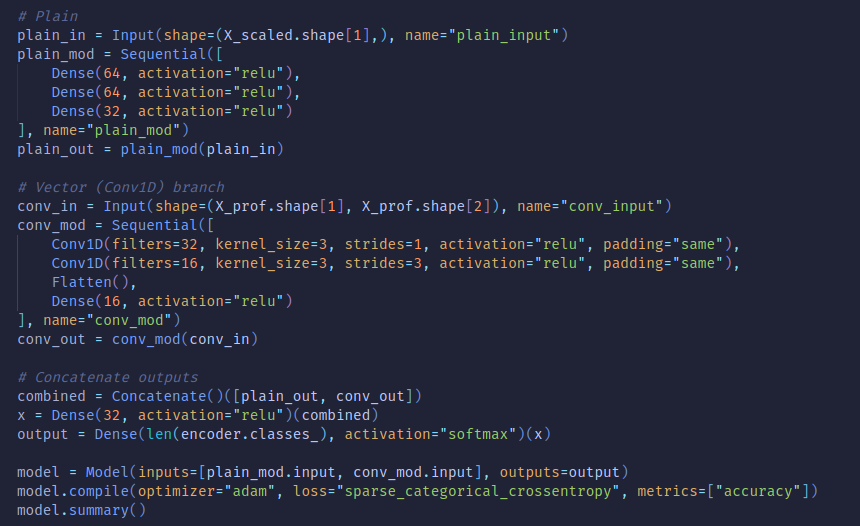
\includegraphics[width=0.8\linewidth]{figures/cnn_model.png}
    \caption{Exemplo de rede CNN1d.}
    \label{fig:cnn}
\end{figure}

Na anterior Subsección tes os documentos base que che permitirán entender o seu funcionamento. O modelo que entrenamos vaise ter que modificar, pois agora imos \textit{concatenar} os resultados de dúas redes: a DNN + a CNN1d. A estrutura é a seguinte:

\begin{itemize}
    \item Un modelo secuencial exactamente igual ao anterior para a parte non convolucional.
    \item Un modelo secuencial para a parte convolucional. Podes probar co da \autoref{fig:cnn} para comezar.

    No código, \verb|filters| é o número de patróns que vai intentar aprender a CNN; \texttt{kernelsize} o número de posicións do vector que se teñen en conta en cada  filtro e \verb|strides| o número de posicións que se despraza o \textit{kernel} entre iteracións. Podes xogar metendo máis layers CNN, cambiando o número de filtros, o tamaño do \textit{kernel}, etc. Tamén podes probar engadindo unha capa de \textit{pooling}. A layer \verb|Flatten| é necesaria para adecuar as dimensións para a seguinte \verb|Dense|, que necesitamos para ter a mesma saída que o modelo DNN.

    \item Concatenamos ambos modelos e superpoñemos máis capas densas para combinar as saídas de ambos modelos. A output é a mesma que anteriormente, coa activación \textit{softmax}. Deberías apreciar unha mellora do \qty{10}{\percent} respecto ao modelo anterior.
\end{itemize}
\subsection{Cuarta semana}
O último paso é amosar unha alternativa ás redes neuronais presentadas. Esta consiste en reconstruír a enerxía cinética de cada partícula no vértice asumindo os tres posibles casos (\textit{p, d, t}) para cada evento e ver cal que hipótese é máis válida dacordo coa cinemática.

Para iso:
\begin{enumerate}
    \item Colle só os eventos que fan punchthrough na segunda capa de silicios (os que queremos identificar). 
    \item Sabendo o espesor dos silicios de \qty{1500}{\mm}, crea unha interpolación para cada partícula: coa función \verb|EnergyLoss.Slow()| garda a $\Delta E_1$ para cada $E_{\text{ini}}$ na entrada do silicio. Podes empregar unha \verb|scipy.CubicSpline| en lugar dunha interpolacion lineal.
    \item Selecciona uns poucos eventos protón. Reconstrúe a súa enerxía no vértice de reacción. Para iso usa a \textit{spline} obtina antes para unha partícula:
    \begin{itemize}
        \item Avalíaa na $\Delta E_1$, obtendo a enerxía á entrada do Si 1.
        \item Utiliza \verb|EnergyLoss| no \textbf{gas} para obter a enerxía de saída da partícula no silicio 0 tras percorrer a distancia \verb|tl_01|. A función \verb|EnergyLoss.EvalInitialEnergy| fai xusto o contrario de \verb|Slow|.
        \item A enerxía á entrada do silicio 0 será a suma $\Delta E_0 + E_{\text{AfterSil0}}$ que acabas de recuperar.
        \item  Por último, calcula a enerxía no vértice (que é onde representas ti a cinemática). Aplica \verb|EvalInitialEnergy| á enerxía anterior pero na distancia entre o silico e o vértice \verb|tl_gas0|.
    \end{itemize}
    \item Con isto obterás un punto $(T, \theta)$ que podes representar sobre un gráfico de cinemática. 
    \item Fai o mesmo asumindo que o evento é \textit{d} e \textit{t}. Represéntaos sobre o mesmo gráfico de cinemática.
    \item Deberías ver como, para un evento \textit{p}, asumir \textit{d} ou \textit{t} leva a un punto que se separa moito de calquera liña cinemática. Só o valor reconstruído como \textit{p} ten sentido.
    \item Deste xeito tes unha identificación. O mesmo aplicará para eventos de deuterio e tritio.
    \item Hai unha aproximación aquí: a interpolación que calculas non depende do ángulo, pero en realidade si que o debería facer, pois a perda de enerxía no silico dependerá do ángulo co que a partícula o atravese (a maior ángulo maior é a distancia que percorre, $d = \qty{1500}{\micro\m}/\cos{\theta}$). Non é necesario que fagas o cálculo tendo en contas isto pero debes sabelo.
    \item Tamén hai unha simplificación: $E_{x} = \qty{0}{\MeV}$ en todo momento. Nun experimento real, o núcleo final \iso{10}{Li} quedará nun estado con enerxía de excitación $E_x$ que fará que a cinemática da partícula lixeira non sexa unha liña senón unha \textit{distribución} no plano. Isto pode complicar a sinxeleza deste método.
\end{enumerate}


\section{Referencias}
\begin{enumerate}
    \item \textit{Hands-on Machine Learning with Scikit-Learn \& Tensorflow}, A. Géron (2017)
    
    É o libro de referencia. A maioría de conceptos están aí definidos, tanto para redes neuronais densas como convolucionais.

    \item \textit{Introduction to Neural Networks}, Y. Zhang \textit{et al.} University of Cornell (2021). Unhas diapositivas interasentes para ter un resumo das NN se non queres ler o libro.
    \item \textit{Neural Networks}, D. Roth \textit{et al.}. University of Pennsylvania (2016). Os capítulos 6 e 7 explican algo máis detalladamente as CNN.
\end{enumerate}

\end{document}
